\documentclass{standalone}
\usepackage{tikz}
\usepackage{ctex,siunitx}
\setCJKmainfont{Noto Serif CJK SC}
\usepackage{tkz-euclide}
\usepackage{amsmath}
\usetikzlibrary{patterns, calc,3d}
\usetikzlibrary {decorations.pathmorphing,decorations.pathreplacing,decorations.shapes}
\begin{document}
\small
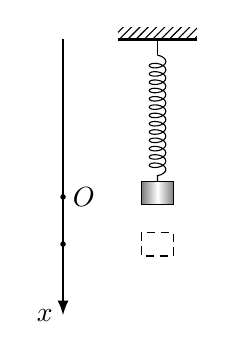
\begin{tikzpicture}[>=latex,scale=1.0]
  \fill[pattern=north east lines](-0.5,0)rectangle(0.5,0.15);
  \draw[thick](-0.5,0)--(0.5,0);
  \draw(0,0)--(0,-0.2);
  \draw[decorate,decoration={coil,segment length=3pt,amplitude=3pt}](0,-0.2)--(0,-1.8);
  \draw[left color=gray,right color=gray,middle color=white](-0.2,-1.8)rectangle(0.2,-2.1);
  \draw[thick,->](-1.2,0)--(-1.2,-3.5)node[left]{$x$};
  \fill(-1.2,-2)circle(1pt)node[right]{$O$};
  \fill(-1.2,-2.6)circle(1pt);
  \draw[densely dashed](-0.2,-2.45)rectangle(0.2,-2.75);
\end{tikzpicture}
\end{document}